\scanpage{104}

\uline{Theorem} \textcircled{1} Let $N$ be a Schatten norm on $R^{(\underline N)}$, \deleted{Let $E$ and $F$ be}\inserted{for every pair $(E,F)$ of} two \deleted{Banach}\inserted{Hilbert} spaces, \deleted{set}\inserted{and} for $u\in L_0(E,F)$, set

\margin{\begin{tikzpicture}[x=1cm,y=1cm]\draw[line width=.2pt] (0,0)--(.03,-.9);\end{tikzpicture}}
\[
N(u)=N((\rho_i(u)))\tag*{(18)}
\]

and for $u\in L(E,F)$

\margin{\begin{tikzpicture}[x=1cm,y=1cm]\draw[line width=.2pt] (0,0)--(.12,-3.3);\end{tikzpicture}}
\[
N(u)=\underset{\substack{v\in F'\otimes E\\N^\circ(u)\leq 1}}{\operatorname{Sup}}|\operatorname{Tr}vu|\tag*{(19)}
\]

This second expression coincides with the preceding one on $L_0(E,F)$. Let $L^N(E,F)$ be the subspace of $L(E,F)$ consisting of the $u$ such that $N(u)<+\infty$, then $N$ is a norm on $L^N(E,F)$, which makes it a Banach space. \deleted{The closure \inserted{$L_N(E,F)$} of $E'\otimes F$ in this \unsure{space is} the space of $u\in L_0(E,F)$ such that} \inserted{If $u\in L_0(E,F)$, then we} have $u\in L^N(E,F)$ if and only if $(\rho_i(u))\in\ell^N$, and then we have (18). \deleted{\unsure{N}} The closure \inserted{$L_N(E,F)$} of $E'\otimes F$ in $L^N(E,F)$ is the set of \deleted{\unsure{compact}} operators $u\in L_0(E,F)$ such that $(\rho_i(u))\in\ell_N$.

\margin{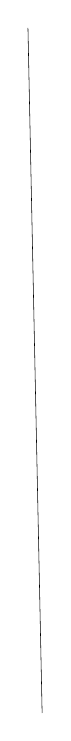
\begin{tikzpicture}[x=1cm,y=1cm]\draw[line width=.2pt] (0,0)--(.18,-8.7);\end{tikzpicture}}
\textcircled{2} We have

\[
\boxed{N(u)=N(u^*)}\boxed{\deleted{\unsure{N(u)}}}\tag*{\textcircled{20}}
\]

and consequently $u\in L^N(E,F)\mathrel{\textcolor{red}{\underline{\textcolor{black}{=}}}}u^*\in L^N(F,E)$
\margin{\deleted{\unsure{$\Longleftrightarrow u\in L^N(E,F)$|on $L^N(E,F)$}}\quad\textcolor{red}{?}}
\inserted{likewise} $u\in L_N^c(E,F)\mathrel{\textcolor{red}{\underline{\textcolor{black}{\Longleftrightarrow}}}}u^*\in L_N(F,E)$. We have

\[
\begin{aligned}
N(uv)&\leq\lVert u\rVert N(v)\\
N(uv)&\leq\lVert v\rVert N(u)
\end{aligned}\tag*{\textcircled{21}}
\]

if $u\in L(E,F)$, $v\in L(F,G)$. \deleted{\unsure{Thus}} By composing on the left or on the right an operator \deleted{$\in L^N($} of type $\ell^N$ (respectively $\ell_N$) with a \deleted{of type} \textcolor{red}{\uline{\textcolor{black}{continuous}}} operator, we obtain an operator of type $\ell^N$ (respectively $\ell_N$).
\margin{\begin{tikzpicture}[x=1cm,y=1cm,line cap=round]\draw[red!70!brown,line width=.4pt] (0,.56)..controls(.015,.47)and(.045,.40)..(.035,.36)..controls(.025,.33)and(.07,.32)..(.075,.35);\draw[red!50!brown,line width=.25pt] (.075,.35)..controls(.16,.37)and(.16,.16)..(.11,.09)..controls(.07,.07)and(.11,.02)..(.10,0)..controls(.11,.04)and(.16,.10)..(.16,.13);\end{tikzpicture}}
\inserted{$N(u)$ is an increasing function on the set of positive Hermitian operators in $L_0(E)$.}

\textcircled{3} \deleted{\textcircled{4}} If $N,N',N''$ are \deleted{\unsure{two|one}}\inserted{some} Schatten norms such that

\[
\text{\unsure{p.|q.}}\qquad\boxed{N(xy)\leq N'(x)N'(y)}\tag*{\textcircled{22}}
\]

for $x,y\in R^{(\underline N)}$, then we have, for $u\in L(E,F)$, $v\in L(F,G)$,

\[
N(vu)\leq \unsure{N'(v)|N'v)}N''(u)\tag*{\textcircled{23}}
\]

thus if $u\in L^{N'}(E,F)$, $v\in L^{N''}(E,F)$, then $vu\in L^N(E,F)$, and if we have \inserted{in addition} $u\in L_{N'}(E,F)$ or $v\in L_{N''}^{\unsure{\deleted{N}|*}}(E,F)$, we will even have $vu\in L_N(E,F)$, -- In particular, we will have, for $u\in L(E,F)$, $v\in L(F,\unsure{G|E})$

\[
\lVert vu\rVert_1\leq N(u)N^\circ(v)\tag*{\textcircled{24}}
\]

thus if $u\in L^N(E,F)$, $v\in L^{N^\circ}(F,\unsure{G|E})$, we have $vu\in L^1(E,\unsure{E|G})$, and

\[
|\operatorname{Tr}vu|\leq N(u)N^\circ(v).\tag*{\textcircled{25}}
\]

\margin{105}
